\subsection*{Teaching Period 1 Progress Report}
\addcontentsline{toc}{subsection}{Teaching Period 1 Progress Report}

This is the teaching period 1 progress review for my final year project, referred to here on after as \textit{Taxicoin}.

\subsubsection*{Current Progress}

As of January 2018, significant progress has been made on the implementation. From a technical point of view, the core ``must have'' features are complete.

As a rider, the user is able to advertise their job to drivers on an individual basis. The intention is that eventually the advertising will be done automatically, to all available drivers which meet some criteria, e.g. minimum rating or maximum proximity from rider.

When accepting a journey with a specific driver, the rider must pay the fare for the journey up-front, as well as an additional deposit which ensures the rider has a stake in completing a journey without dispute.

At the end of a journey, the rider is able to rate the driver. The rating acts as the only form of reputation, and is currently a simple average of all ratings. Each rating is an integer between 1 and 5.

Drivers are able to advertise their location publicly as an indication that they are active and accepting job proposals. However, to do so, drivers must provide a deposit.

In the event that a driver receives a job proposal, they have the option to respond with a quote for the fare of the journey.

\subsubsection*{Significant Achievements}

\begin{itemize}
    \item Technical contract implementation is now in a working state.
    \item User interface with map, location search, and user geolocation is in a working state.
    \item Spoke at BrumJS November 2017 meetup on the subject of the Ethereum platform and its uses. Afterwards gathered informal feedback about the concept of Taxicoin.
\end{itemize}

\subsubsection*{Next Steps}

In terms of the implementation itself, the user interface needs tidying up significantly. At the moment, the ``user flow'' is somewhat lacking, and not as fluid as it should be. This is the first priority.

The reputation is currently very simplified from what I had initially planned. I would like to develop it further, as it is an integral part of the application. I've recently read into how other Ethereum-based decentralised applications are managing their reputation systems, and will hopefully apply some of the ideas in Taxicoin.

I plan to write an ``Introduction to Ethereum'' section of the report, with a comprehensive explanation of how the platform functions, and why I have chosen to develop Taxicoin with it.

As discussed with Peter Lewis, a crucial part in proving the successful implementation of a complete protocol for Taxicoin will be to develop a comprehensive suite of tests. These will primarily test the functionality of the contract parts of the application, as this is where the protocol layer is implemented.

\subsubsection*{Hurdles}

The Ethereum platform is still rapidly evolving. Indeed, even from when I began research into how I would develop this project, protocol specifications have been amended. As a result, I am having to keep an eye on developments with Ethereum while developing the application.

Traditional databases for storing data do not translate well to blockchain-based systems. Therefore I will need to research distributed databases, particularly for a more advanced reputation system. This is unexplored territory for me, so I am unsure what to expect.

\subsubsection*{Project Diary}

\begin{description}
    \item[3rd October 2017] talked about the fact that this project is relevant to the interests of the ALICE group. It is effectively a self-governing application. Was decided that the focus should be on compiling a list of ``must have'' features and then implementing them.
    \item[16th October 2017] was suggested to write a RFC-style protocol specification, to be used later to test against to determine if the implementation is correct.
    \item[13th November 2017] no huge amount of progress was reported due to other commitments. We revisited the idea of producing an RFC-style document, focusing on the IMAP protocol as an example.
    \item[4th December 2017] we discussed that including a network architecture diagram in the report would be a good idea of explaining how various parts of the project communicate with each other (e.g. front end talks to contract, different instances of front end talk to each other). At this point, a working implementation had been completed, therefore we began talking about how to write tests. It was decided that the contract should be tested directly with unit tests, and potentially integration testing performed on the Javascript abstraction layer and contract. We discussed that it would be good to get to the point where the application could be security audited.
\end{description}

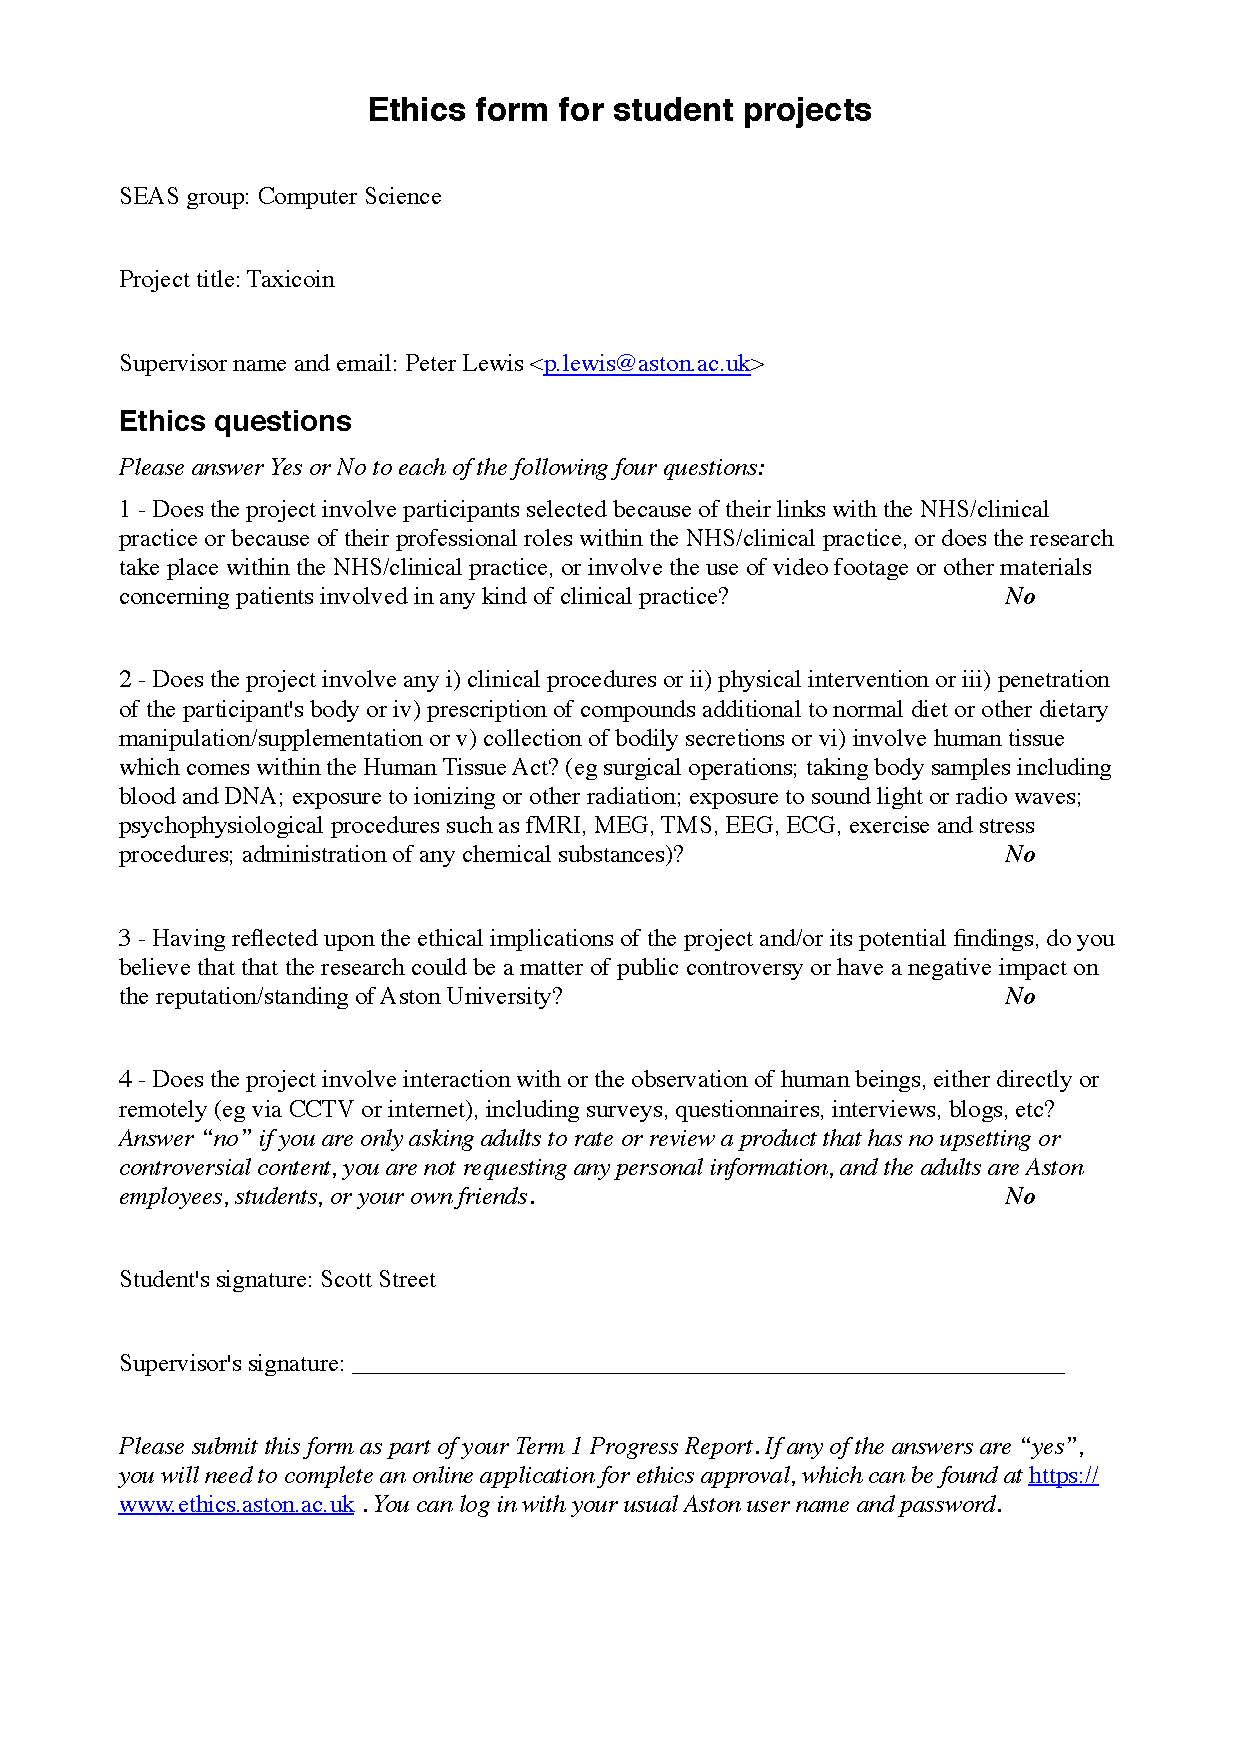
\includepdf[pages={1}]{res/ethics.pdf}
